\documentclass[a4paper,11pt,eval]{nsi} 

\usepackage{pifont}
\usepackage{fontawesome5}
%\pagestyle{empty}


\newcounter{exoNum}
\setcounter{exoNum}{0}
%
\newcommand{\exo}[1]
{
	\addtocounter{exoNum}{1}
	{\titlefont\color{UGLiBlue}\Large Exercice\ \theexoNum\ \normalsize{#1}}\smallskip	
}



\begin{document}



\textcolor{UGLiBlue}{Vendredi 25/04/2025}\\
\classe{\premiere spé}
\titre{Interrogation de cours - Sujet B}
\maketitle
\begin{center}
	Calculatrice interdite
\end{center}
Pour chaque expression, placer le point $M_i$ correspondant à la valeur de l'angle sur le cercle trigonométrique et donner la valeur exacte :\\

\dleft{6cm}{
    \begin{enumerate}[itemsep=1em]
        \item \begin{minipage}[t]{\linewidth} $\cos\left(\dfrac{\pi}{2}\right)$ \end{minipage}
	\item \begin{minipage}[t]{\linewidth} $\cos\left(-\dfrac{\pi}{4}\right)$ \end{minipage}
	\item \begin{minipage}[t]{\linewidth} $\cos\left(-\dfrac{\pi}{2}\right)$ \end{minipage}
	\item \begin{minipage}[t]{\linewidth} $\sin\left(\dfrac{3\pi}{4}\right)$ \end{minipage}
	\item \begin{minipage}[t]{\linewidth} $\cos\left(\dfrac{2\pi}{3}\right)$ \end{minipage}
	\item \begin{minipage}[t]{\linewidth} $\sin\left(\dfrac{5\pi}{6}\right)$ \end{minipage}
	\item \begin{minipage}[t]{\linewidth} $\sin\left(-\dfrac{\pi}{4}\right)$ \end{minipage}
	\item \begin{minipage}[t]{\linewidth} $\cos\left(\dfrac{\pi}{6}\right)$ \end{minipage}
	\item \begin{minipage}[t]{\linewidth} $\sin\left(\dfrac{\pi}{2}\right)$ \end{minipage}
	\item \begin{minipage}[t]{\linewidth} $\sin\left(3\pi\right)$ \end{minipage}
\end{enumerate}
}
{
    \begin{tikzpicture}[scale = 4.5]	
		\draw 	(0,0) circle(1);
		
		\draw[dashed]   (150:1)--(030:1)\ball--(330:1)\ball--(210:1)\ball--(150:1)\ball;
        \draw[dashed]   (45:1)--(135:1)\ball--(225:1)\ball--(315:1)\ball--(45:1)\ball;
        \draw[dashed]   (60:1)--(120:1)\ball--(240:1)\ball--(300:1)\ball--(60:1)\ball;
        

        \draw   (0,0)--(000:1)\ball;
		\draw   (0,0)--(090:1)\ball;
		\draw   (0,0)--(180:1)\ball;
		\draw   (0,0)--(270:1)\ball;
		
		\draw   (000:1.2) node{I};
		%\draw   (030:1.2) node{$M\left(\dfrac{\pi}{6}\right)$};
		%\draw   (045:1.2) node{$M\left(\dfrac{\pi}{4}\right)$};
		%\draw   (060:1.2) node{$M\left(\dfrac{\pi}{3}\right)$};
		\draw   (090:1.2) node{J};
		
		\draw (0,0) node[below left]{O};
	\end{tikzpicture}
}

\newpage
\begin{multicols}{2}

\begin{enumerate}[itemsep=1em]
    \item \begin{minipage}[t]{\linewidth}$\cos\left(\dfrac{\pi}{2}\right)=0$

        \medskip
        \begin{tikzpicture}[baseline,scale = 0.5]
        
            \tikzset{
              point/.style={
                thick,
                draw,
                cross out,
                inner sep=0pt,
                minimum width=5pt,
                minimum height=5pt,
              },
            }
            \clip (-8,-6.8) rectangle (8,6.8);
                \draw[color={black},fill opacity = 1.1] (0,0) circle (5);
            \draw (0,6.151544993495972) node[anchor = center] {\colorbox {white}{\footnotesize  \color{black}{$\dfrac{\pi}{2}$}}};
            \draw[color={blue},line width = 3] (0,0)--(0.8,0)--(0.8,0.8)--(0,0.8)--cycle;
            \draw[color ={black}] (5,0)--(-5,0);
            \draw[color ={black}] (0,5)--(0,-5);
            \draw (0,-1.0484550065040281) node[anchor = center] {\colorbox {white}{\footnotesize  \color{black}{$0$}}};
            \draw[color ={black},line width = 3] (0,0)--(0,0);
            \draw[color ={black}, dashed ] (0,5)--(0,0);
            \draw[color ={blue},line width = 3] (0,0)--(0,5);
            \draw[color ={blue},line width = 3] (0,0)--(5,0);
        
        \end{tikzpicture}\\
        \end{minipage}
        \item \begin{minipage}[t]{\linewidth}$\cos\left(-\dfrac{\pi}{4}\right)=\dfrac{\sqrt{2}}{2}$
        
        \medskip
        \begin{tikzpicture}[baseline,scale = 0.5]
        
            \tikzset{
              point/.style={
                thick,
                draw,
                cross out,
                inner sep=0pt,
                minimum width=5pt,
                minimum height=5pt,
              },
            }
            \clip (-8,-6.8) rectangle (8,6.8);
                \draw[color={black},fill opacity = 1.1] (0,0) circle (5);
            \draw (4.03,-3.5784550065040284) node[anchor = center] {\colorbox {white}{\footnotesize  \color{black}{$-\dfrac{\pi}{4}$}}};
            \draw[color={black}] (0.8,0) arc (0:-45:0.8) ;
            \draw[color ={black}] (5,0)--(-5,0);
            \draw[color ={black}] (0,5)--(0,-5);
            \draw (3.54,1.9515449934959719) node[anchor = center] {\colorbox {white}{\footnotesize  \color{black}{$\dfrac{\sqrt{2}}{2}$}}};
            \draw[color ={black},line width = 3] (0,0)--(3.54,0);
            \draw[color ={black}, dashed ] (3.54,-3.54)--(3.54,0);
            \draw[color ={blue},line width = 3] (0,0)--(3.54,-3.54);
            \draw[color ={blue},line width = 3] (0,0)--(5,0);
        
        \end{tikzpicture}\\
        \end{minipage}
        \item \begin{minipage}[t]{\linewidth}$\cos\left(-\dfrac{\pi}{2}\right)=0$
        
        \medskip
        \begin{tikzpicture}[baseline,scale = 0.5]
        
            \tikzset{
              point/.style={
                thick,
                draw,
                cross out,
                inner sep=0pt,
                minimum width=5pt,
                minimum height=5pt,
              },
            }
            \clip (-8,-6.8) rectangle (8,6.8);
                \draw[color={black},fill opacity = 1.1] (0,0) circle (5);
            \draw (0,-5.248455006504028) node[anchor = center] {\colorbox {white}{\footnotesize  \color{black}{$-\dfrac{\pi}{2}$}}};
            \draw[color={blue},line width = 3] (0,0)--(0.8,0)--(0.8,-0.8)--(0,-0.8)--cycle;
            \draw[color ={black}] (5,0)--(-5,0);
            \draw[color ={black}] (0,5)--(0,-5);
            \draw (0,1.9515449934959719) node[anchor = center] {\colorbox {white}{\footnotesize  \color{black}{$0$}}};
            \draw[color ={black},line width = 3] (0,0)--(0,0);
            \draw[color ={black}, dashed ] (0,-5)--(0,0);
            \draw[color ={blue},line width = 3] (0,0)--(0,-5);
            \draw[color ={blue},line width = 3] (0,0)--(5,0);
        
        \end{tikzpicture}\\
        \end{minipage}
        \item \begin{minipage}[t]{\linewidth}$\sin\left(\dfrac{3\pi}{4}\right)=\dfrac{\sqrt{2}}{2}$
        
        \medskip
        \begin{tikzpicture}[baseline,scale = 0.5]
        
            \tikzset{
              point/.style={
                thick,
                draw,
                cross out,
                inner sep=0pt,
                minimum width=5pt,
                minimum height=5pt,
              },
            }
            \clip (-8,-6.8) rectangle (8,6.8);
                \draw[color={black},fill opacity = 1.1] (0,0) circle (5);
            \draw (-4.03,4.481544993495972) node[anchor = center] {\colorbox {white}{\footnotesize  \color{black}{$\dfrac{3\pi}{4}$}}};
            \draw[color={black}] (0.8,0) arc (0:135:0.8) ;
            \draw[color ={black}] (5,0)--(-5,0);
            \draw[color ={black}] (0,5)--(0,-5);
            \draw (0.65,3.991544993495972) node[anchor = center] {\colorbox {white}{\footnotesize  \color{black}{$\dfrac{\sqrt{2}}{2}$}}};
            \draw[color ={black},line width = 3] (0,0)--(0,3.54);
            \draw[color ={black}, dashed ] (-3.54,3.54)--(0,3.54);
            \draw[color ={blue},line width = 3] (0,0)--(-3.54,3.54);
            \draw[color ={blue},line width = 3] (0,0)--(5,0);
        
        \end{tikzpicture}\\
        \end{minipage}
        \item \begin{minipage}[t]{\linewidth}$\cos\left(\dfrac{2\pi}{3}\right)=-\dfrac{1}{2}$
        
        \medskip
        \begin{tikzpicture}[baseline,scale = 0.5]
        
            \tikzset{
              point/.style={
                thick,
                draw,
                cross out,
                inner sep=0pt,
                minimum width=5pt,
                minimum height=5pt,
              },
            }
            \clip (-8,-6.8) rectangle (8,6.8);
                \draw[color={black},fill opacity = 1.1] (0,0) circle (5);
            \draw (-2.85,5.391544993495972) node[anchor = center] {\colorbox {white}{\footnotesize  \color{black}{$\dfrac{2\pi}{3}$}}};
            \draw[color={black}] (0.8,0) arc (0:120:0.8) ;
            \draw[color ={black}] (5,0)--(-5,0);
            \draw[color ={black}] (0,5)--(0,-5);
            \draw (-2.5,-1.0484550065040281) node[anchor = center] {\colorbox {white}{\footnotesize  \color{black}{$-\dfrac{1}{2}$}}};
            \draw[color ={black},line width = 3] (0,0)--(-2.5,0);
            \draw[color ={black}, dashed ] (-2.5,4.33)--(-2.5,0);
            \draw[color ={blue},line width = 3] (0,0)--(-2.5,4.33);
            \draw[color ={blue},line width = 3] (0,0)--(5,0);
        
        \end{tikzpicture}\\
        \end{minipage}
        \item \begin{minipage}[t]{\linewidth}$\sin\left(\dfrac{5\pi}{6}\right)=\dfrac{1}{2}$
        
        \medskip
        \begin{tikzpicture}[baseline,scale = 0.5]
        
            \tikzset{
              point/.style={
                thick,
                draw,
                cross out,
                inner sep=0pt,
                minimum width=5pt,
                minimum height=5pt,
              },
            }
            \clip (-8,-6.8) rectangle (8,6.8);
                \draw[color={black},fill opacity = 1.1] (0,0) circle (5);
            \draw (-4.94,3.301544993495972) node[anchor = center] {\colorbox {white}{\footnotesize  \color{black}{$\dfrac{5\pi}{6}$}}};
            \draw[color={black}] (0.8,0) arc (0:150:0.8) ;
            \draw[color ={black}] (5,0)--(-5,0);
            \draw[color ={black}] (0,5)--(0,-5);
            \draw (0.65,2.951544993495972) node[anchor = center] {\colorbox {white}{\footnotesize  \color{black}{$\dfrac{1}{2}$}}};
            \draw[color ={black},line width = 3] (0,0)--(0,2.5);
            \draw[color ={black}, dashed ] (-4.33,2.5)--(0,2.5);
            \draw[color ={blue},line width = 3] (0,0)--(-4.33,2.5);
            \draw[color ={blue},line width = 3] (0,0)--(5,0);
        
        \end{tikzpicture}\\
        \end{minipage}
        \item \begin{minipage}[t]{\linewidth}$\sin\left(-\dfrac{\pi}{4}\right)=-\dfrac{\sqrt{2}}{2}$
        
        \medskip
        \begin{tikzpicture}[baseline,scale = 0.5]
        
            \tikzset{
              point/.style={
                thick,
                draw,
                cross out,
                inner sep=0pt,
                minimum width=5pt,
                minimum height=5pt,
              },
            }
            \clip (-8,-6.8) rectangle (8,6.8);
                \draw[color={black},fill opacity = 1.1] (0,0) circle (5);
            \draw (4.03,-3.5784550065040284) node[anchor = center] {\colorbox {white}{\footnotesize  \color{black}{$-\dfrac{\pi}{4}$}}};
            \draw[color={black}] (0.8,0) arc (0:-45:0.8) ;
            \draw[color ={black}] (5,0)--(-5,0);
            \draw[color ={black}] (0,5)--(0,-5);
            \draw (-1.5,-3.088455006504028) node[anchor = center] {\colorbox {white}{\footnotesize  \color{black}{$-\dfrac{\sqrt{2}}{2}$}}};
            \draw[color ={black},line width = 3] (0,0)--(0,-3.54);
            \draw[color ={black}, dashed ] (3.54,-3.54)--(0,-3.54);
            \draw[color ={blue},line width = 3] (0,0)--(3.54,-3.54);
            \draw[color ={blue},line width = 3] (0,0)--(5,0);
        
        \end{tikzpicture}\\
        \end{minipage}
        \item \begin{minipage}[t]{\linewidth}$\cos\left(\dfrac{\pi}{6}\right)=\dfrac{\sqrt{3}}{2}$
        
        \medskip
        \begin{tikzpicture}[baseline,scale = 0.5]
        
            \tikzset{
              point/.style={
                thick,
                draw,
                cross out,
                inner sep=0pt,
                minimum width=5pt,
                minimum height=5pt,
              },
            }
            \clip (-8,-6.8) rectangle (8,6.8);
                \draw[color={black},fill opacity = 1.1] (0,0) circle (5);
            \draw (4.94,3.301544993495972) node[anchor = center] {\colorbox {white}{\footnotesize  \color{black}{$\dfrac{\pi}{6}$}}};
            \draw[color={black}] (0.8,0) arc (0:30:0.8) ;
            \draw[color ={black}] (5,0)--(-5,0);
            \draw[color ={black}] (0,5)--(0,-5);
            \draw (4.33,-1.0484550065040281) node[anchor = center] {\colorbox {white}{\footnotesize  \color{black}{$\dfrac{\sqrt{3}}{2}$}}};
            \draw[color ={black},line width = 3] (0,0)--(4.33,0);
            \draw[color ={black}, dashed ] (4.33,2.5)--(4.33,0);
            \draw[color ={blue},line width = 3] (0,0)--(4.33,2.5);
            \draw[color ={blue},line width = 3] (0,0)--(5,0);
        
        \end{tikzpicture}\\
        \end{minipage}
        \item \begin{minipage}[t]{\linewidth}$\sin\left(\dfrac{\pi}{2}\right)=1$
        
        \medskip
        \begin{tikzpicture}[baseline,scale = 0.5]
        
            \tikzset{
              point/.style={
                thick,
                draw,
                cross out,
                inner sep=0pt,
                minimum width=5pt,
                minimum height=5pt,
              },
            }
            \clip (-8,-6.8) rectangle (8,6.8);
                \draw[color={black},fill opacity = 1.1] (0,0) circle (5);
            \draw (0,6.151544993495972) node[anchor = center] {\colorbox {white}{\footnotesize  \color{black}{$\dfrac{\pi}{2}$}}};
            \draw[color={blue},line width = 3] (0,0)--(0.8,0)--(0.8,0.8)--(0,0.8)--cycle;
            \draw[color ={black}] (5,0)--(-5,0);
            \draw[color ={black}] (0,5)--(0,-5);
            \draw (-1.5,5.451544993495972) node[anchor = center] {\colorbox {white}{\footnotesize  \color{black}{$1$}}};
            \draw[color ={black},line width = 3] (0,0)--(0,5);
            
            \draw[color ={blue},line width = 3] (0,0)--(0,5);
            \draw[color ={blue},line width = 3] (0,0)--(5,0);
        
        \end{tikzpicture}\\
        \end{minipage}
        \item \begin{minipage}[t]{\linewidth}$\sin\left(3\pi\right)=0$
        
        \medskip
        \begin{tikzpicture}[baseline,scale = 0.5]
    
            \tikzset{
              point/.style={
                thick,
                draw,
                cross out,
                inner sep=0pt,
                minimum width=5pt,
                minimum height=5pt,
              },
            }
            \clip (-8,-6.8) rectangle (8,6.8);
                \draw[color={black},fill opacity = 1.1] (0,0) circle (5);
            \draw (-6.151544993495972,0) node[anchor = center] {\colorbox {white}{\footnotesize  \color{black}{$3\pi$}}};
            %\draw[color={blue},line width = 3] (0,0)--(0.8,0)--(0.8,0.8)--(0,0.8)--cycle;
            \draw[color ={black}] (5,0)--(-5,0);
            \draw[color ={black}] (0,5)--(0,-5);
            \draw (0,-1.0484550065040281) node[anchor = center] {\colorbox {white}{\footnotesize  \color{black}{$0$}}};
            %\draw (-5,-1.0484550065040281) node[anchor = center] {\colorbox {white}{\footnotesize  \color{black}{$-1$}}};
            \draw[color ={black},line width = 3] (0,0)--(0,0);
            %\draw[color ={black}, dashed ] (0,5)--(0,0);
            \draw[color ={blue},line width = 3] (-5,0)--(5,0);
            %\draw[color ={blue},line width = 3] (0,0)--(5,0);
        
        \end{tikzpicture}\\
        \end{minipage}
        \end{enumerate}
    \end{multicols}
\end{document}
